\documentclass[../../full]{subfiles}


\begin{document}
    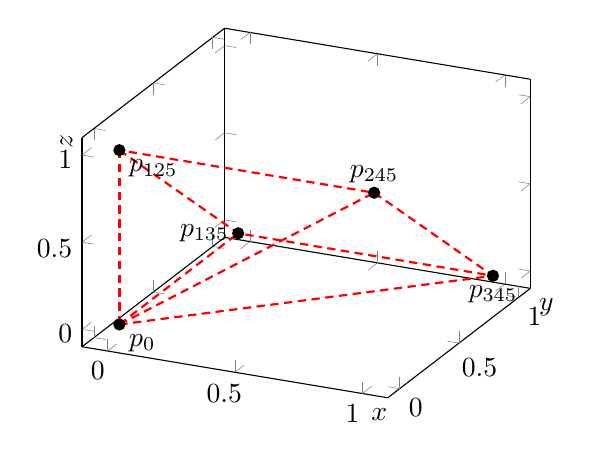
\begin{tikzpicture}
        \begin{axis}[
            width=0.6\textwidth,
            view={25}{30},
            xlabel={\( x \)},
            ylabel={\( y \)},
            zlabel={\( z \)},
            xmin=0, xmax=1,
            ymin=0, ymax=1,
            zmin=0, zmax=1,
            enlargelimits=0.1,
            every axis x label/.append style={at=(ticklabel* cs:1)},
            every axis y label/.append style={at=(ticklabel* cs:1)},
            every axis z label/.append style={at=(ticklabel* cs:1)},
        ]
            \def\A{(0, 0, 0)}
            \def\B{(0, 0, 1)}
            \def\C{(0, 1, 0)}
            \def\D{(1, 0, 1)}
            \def\E{(1, 1, 0)}
            %
            \addplot3 [only marks] coordinates {\A \B \C \D \E};
            %
            \addplot3 [Red, thick, no marks, densely dashed] coordinates
                {\B \C \E \D \B};
            \addplot3 [Red, thick, no marks, densely dashed] coordinates
                {\A \B};
            \addplot3 [Red, thick, no marks, densely dashed] coordinates
                {\A \C};
            \addplot3 [Red, thick, no marks, densely dashed] coordinates
                {\A \D};
            \addplot3 [Red, thick, no marks, densely dashed] coordinates
                {\A \E};
            %
            \node [below right] at (axis cs: 0, 0, 0) {\( p_0 \)};
            \node [below right] at (axis cs: 0, 0, 1) {\( p_{125} \)};
            \node [left] at (axis cs: 0, 1, 0) {\( p_{135} \)};
            \node [above] at (axis cs: 1, 0, 1) {\( p_{245} \)};
            \node [below] at (axis cs: 1, 1, 0) {\( p_{345} \)};
        \end{axis}
    \end{tikzpicture}
\end{document}
